\section{Model ODFs}


\subsection*{ODFs in MTEX}


\begin{frame}[fragile]
  \frametitle{Orientation Density Functions in \MTEX}


  \centering{
    \includegraphics[width=10cm]{latex_pic/odf}
  }

\end{frame}

\subsection*{ODFs in MTEX}


\subsection*{The Class kernel}


\begin{frame}[fragile]
  \frametitle{The Shape of the ODF -- The \MTEX Class \texttt{\bf kernel}}

Definition:

\begin{lstlisting}
psi = kernel('de la Vallee Poussin',80);
psi = kernel('Abel Poisson','halfwidth',10*degree);
\end{lstlisting}

\medskip

Supported kernel functions:

\begin{quote}
  Abel -- Poisson, de la Vall\'ee Poussin, von Mises -- Fisher, fibre von Mises
  -- Fisher, Gauss -- Weierstrass, Dirichlet, Bump
\end{quote}

Plot of the \textcolor{blue}{Abel Poisson}, the \textcolor{red}{Dirichlet} and
the \textcolor{green}{Bump} kernel:

\onslide<1->
\begin{center}
  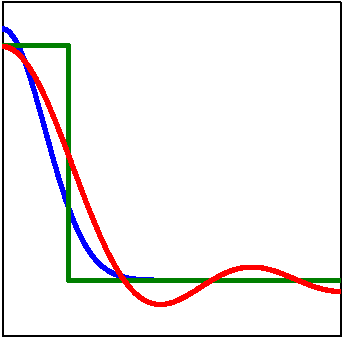
\includegraphics[width=3.5cm]{pic/K} \quad
  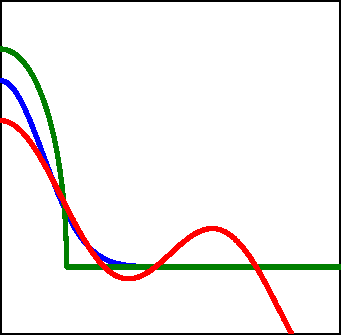
\includegraphics[width=3.5cm]{pic/RK} \quad
  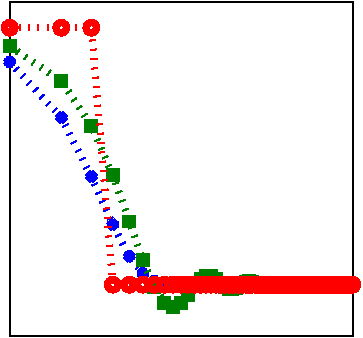
\includegraphics[width=3.5cm]{pic/Fourier}
\end{center}

\end{frame}

\subsection*{Unimodal ODFs}

\begin{frame}[fragile]
  \frametitle{Defining Unimodal ODFs in \MTEX}

\begin{columns}

  \begin{column}{8.5cm}

      Characteristics of an unimodal ODF:
      \begin{enumerate}
      \item crystal symmetry
      \item specimen symmetry
      \item modal orientation
      \item kernel function
      \end{enumerate}



\begin{lstlisting}
SS = symmetry('orthorhombic')
CS = symmetry('cubic')
q = Miller2quat([1 2 2],[2 2 1],CS);
psi = kernel('von Mises Fisher',...
             'halfwidth',20*degree);
\end{lstlisting}

      \begin{actionenv}<1-| alert@1->
\begin{lstlisting}
odf = unimodalODF(q,CS,SS,psi)
\end{lstlisting}
    \end{actionenv}

\end{column}

    \begin{column}{3cm}
      \onslide<1->
      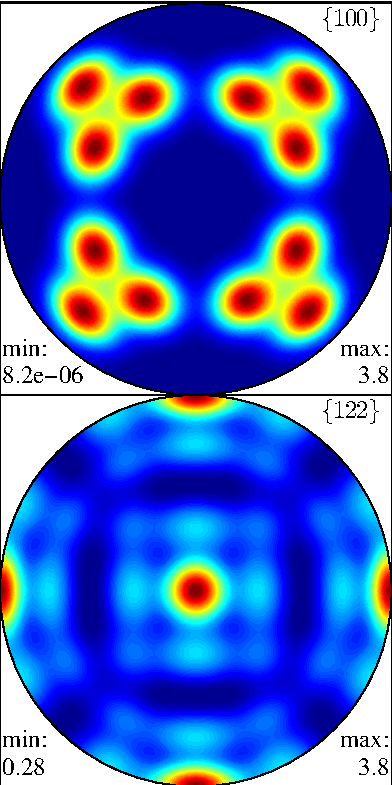
\includegraphics[width=3cm]{pic/unimodalODF}
    \end{column}
  \end{columns}

\end{frame}



\subsection*{Fibre ODFs}

\begin{frame}[fragile]
  \frametitle{Defining Fibre ODFs in \MTEX}

  \begin{columns}

    \begin{column}{8.5cm}

      Characteristics of an Fibre ODFs:
      \begin{enumerate}
      \item crystal symmetry
      \item specimen symmetry
      \item crystal direction
      \item specimen direction
      \item kernel function
      \end{enumerate}


\begin{lstlisting}
SS = symmetry('triclinic')
CS = symmetry('hexagonal')
h = Miller(1,0,0,CS);
r = xvector;
psi = kernel('Abel Poisson',...
             'halfwidth',18*degree);
\end{lstlisting}

      \begin{actionenv}<1-| alert@1->
\begin{lstlisting}
odf = fibreODF(h,r,CS,SS,psi)
\end{lstlisting}
      \end{actionenv}

\end{column}

    \begin{column}{3cm}
      \onslide<1->
      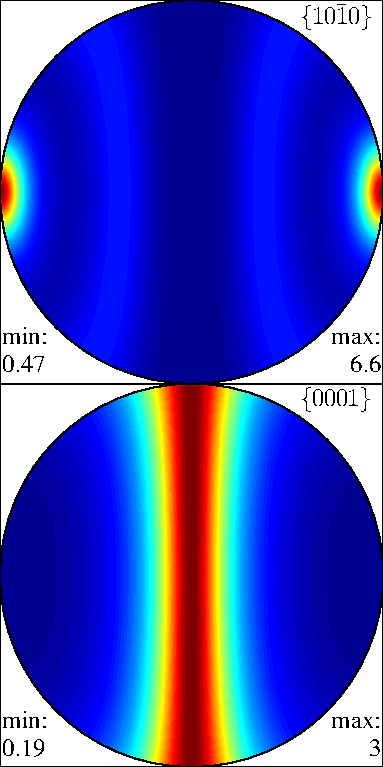
\includegraphics[width=3cm]{pic/fibreODF}
    \end{column}
  \end{columns}


\end{frame}

\subsection*{Fourier ODFs}

\begin{frame}[fragile]
  \frametitle{Defining Uniform and  Fourier ODFs}

  The uniform ODF:
\begin{lstlisting}
SS = symmetry('triclinic')
CS = symmetry('hexagonal')
\end{lstlisting}

  \begin{actionenv}<1-| alert@1->
\begin{lstlisting}
 odf = uniformODF(CS,SS)
\end{lstlisting}
  \end{actionenv}

  \begin{block}{Fourier expansion of an ODF}
    \begin{equation*}
      f(\vec g) = \sum_{l=0}^L \sum_{k,k'=-l}^l C_l^{k,k'} T_l^{k,k'}(\vec g)
    \end{equation*}
    \begin{equation*}
      C = [C_0,C_1^{-1,-1},C_1^{0,-1},C_1^{1,-1},\ldots,C_1^{1,1},C_2^{-2,-2},\ldots,C_L^{L,L}]
    \end{equation*}
  \end{block}
The Fourier ODF:
  \begin{actionenv}<1-| alert@1->
\begin{lstlisting}
odf = FourierODF(C,CS,SS)
\end{lstlisting}
  \end{actionenv}



\end{frame}

\subsection*{ODF Arithmetic}

\begin{frame}[fragile]
  \frametitle{ODF Arithmetic}


  \begin{columns}
    \begin{column}{6cm}

      Calculate with ODFs:
\begin{lstlisting}
odf1 = unimodalODF(...)
odf2 = fibreODF(...)
odf3 = uniformODF(CS,SS)

odf = 0.2*odf1 + 0.3*odf2
      + 0.5*odf3

\end{lstlisting}

  Rotate ODFs:
\begin{lstlisting}
q = axis2quat(xvector,...
              90*degree);
odf = rotate(odf,q)
\end{lstlisting}


  Standard ODFs:
\begin{lstlisting}
odf = santafee;
\end{lstlisting}


\end{column}
\begin{column}{5cm}
  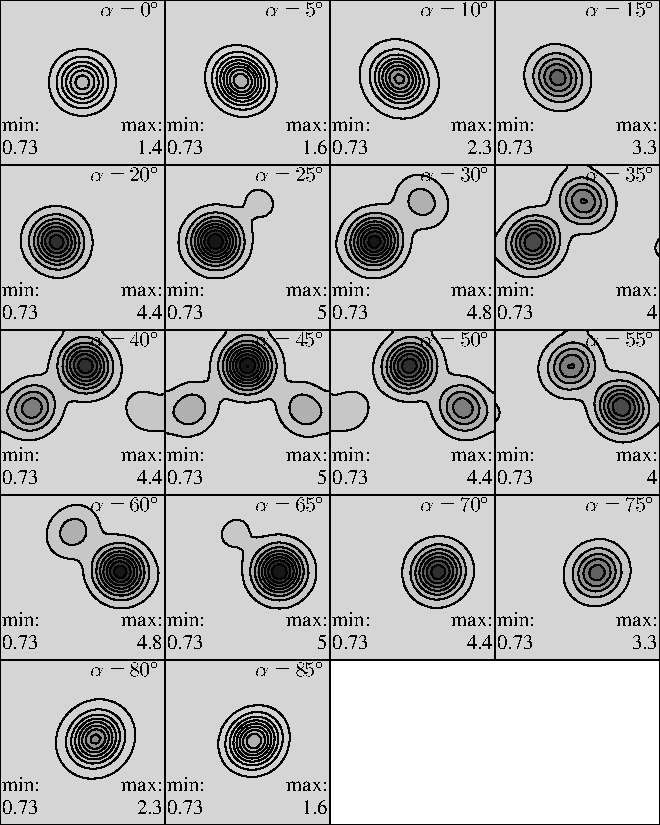
\includegraphics[width=5cm]{pic/santafeeh}
\end{column}
\end{columns}

\end{frame}

%%% Local Variables:
%%% mode: latex
%%% TeX-master: "main"
%%% End:
